% Популяционный анализ представлений импульсной сети (перенесён из MANGO/Гл.3 в Гл.2:
% это популяционный уровень — размерность, информационная плоскость).
% Связь MI<->MEI осталась в MANGO (sec:ib_mei), ссылается сюда назад.

\section{Геометрия и информационное содержание представлений импульсной нейронной сети}\label{sec:snn_population}

% \link{Связка: тот же аппарат снижения и оценки размерности, что применялся к популяционной активности гиппокампа и к рекуррентной сети, приложим и к импульсным сетям — это демонстрирует субстрат-независимость инструментария.}
Аппарат снижения размерности и оценки размерности, применённый выше к популяционной активности гиппокампа (секция~\ref{sec:dim}) и к рекуррентной нейронной сети (секция~\ref{sec:rnn}), приложим и к импульсным нейронным сетям. В данной секции коллективная динамика представлений импульсной сети анализируется на протяжении обучения~--- с точки зрения геометрии и информационного содержания.

Анализировалась импульсная сеть ResNet-18 с нейронами с утечкой и накоплением (LIF), обученная классификации CIFAR-10 (полное описание сети и процедуры обучения~--- в разделе про синтез оптимальных стимулов, секция~\ref{sec:mango}). В качестве данных использовалось суммарное число спайков каждого нейрона по $T=50$ временным шагам для $10\,000$ тестовых изображений CIFAR-10. Анализ проведён для всех 17 спайковых слоёв на 26~эпохах обучения (от~0 до~900), что покрывает полную траекторию обучения. Число нейронов варьировалось от 64 (layer1) до 512 (layer4). Все вычисления выполнены с помощью пакета DRIADA (секция~\ref{sec:driada}).

\paragraph{Меры размерности.}
Для характеризации геометрии представлений использовались эффективная размерность (ЭР) и внутренняя размерность (ВР), подробно описанные в секции~\ref{sec:dim}. ЭР~--- квадратичная энтропия Реньи спектра корреляционной матрицы с итеративной коррекцией Марченко--Пастура~--- отражает число значимых линейных компонент. ВР~--- оценщик 2-NN~--- отражает локальную геометрическую размерность данных на многообразии. Обе меры вычислены через DRIADA (\texttt{eff\_dim} и \texttt{nn\_dimension}) с теми же параметрами, что и при анализе кальциевых данных гиппокампа, что обеспечивает прямую сопоставимость результатов между биологической и искусственной нейронной сетью.

\paragraph{Оценка взаимной информации.}
Для количественной оценки информации о классах, содержащейся в активности каждого слоя, были использованы три уровня оценки взаимной информации $I(T; Y)$, где $T$~--- вектор активности слоя, $Y$~--- метки классов.

\begin{enumerate}
    \item \textit{Попарная MI}: $I_{ind} = \sum_i I(t_i; Y)$~--- сумма точных дискретных MI отдельных нейронов с метками. Не учитывает корреляции между нейронами и является верхней оценкой уникальной информации.
    \item \textit{Гауссово приближение}: $I_{gauss}$~--- копула-энтропия GCMI из DRIADA (\texttt{mi\_model\_gd}). Учитывает попарные корреляции между нейронами; отношение $I_{gauss}/I_{ind}$ характеризует степень избыточности кодирования.
    \item \textit{Нелинейная оценка через сжатие}: автоэнкодер со вспомогательной классификационной задачей сжимает активность слоя в 16-мерное латентное пространство~$Z$, после чего $I(Z; Y)$ оценивается непараметрическим KSG-оценщиком. Это нижняя граница на~$I(T; Y)$, контролируемая точностью классификации из~$Z$.
\end{enumerate}

Классификационная задача автоэнкодера реализована как дополнительный компонент лосс-системы DRIADA (\texttt{ClassificationLoss} в модуле \texttt{dim\_reduction.losses}): модель одновременно минимизирует ошибку реконструкции и кросс-энтропийный лосс, что гарантирует сохранение классовой информации при сжатии. Качество сжатия контролировалось: для layer2--4 точность классификации из~$Z$ не уступала точности из полного~$T$.

Все оценки взаимной информации скорректированы на смещение оценщика вычитанием значения, полученного на перемешанных метках классов: $I_{corrected} = I_{raw} - I_{shuffle}$. Это устраняет конечновыборочное смещение, систематически завышающее оценки MI.

\paragraph{Информационная плоскость.}
Информационная плоскость~\cite{ShwartzZiv2017} строится как $H_{gauss}(T)$ по горизонтальной и $I(Z; Y)$ по вертикальной оси, где $H_{gauss}(T) = \frac{1}{2}\sum_k \log_2(2\pi e \lambda_k)$~--- гауссова верхняя граница энтропии активности слоя. Для детерминированной сети $I(X; T) = H(T)$, так что $H_{gauss}$ может рассматриваться как приближение $I(X; T)$. Каждая точка на плоскости соответствует одному слою на одной эпохе; стрелки показывают направление обучения.

%========================================================================
\subsection{Геометрия представлений: профили размерности}\label{sec:ib_geometry}

Профиль ВР по слоям обученной импульсной сети (эпоха~900) имеет характерную форму горба (hunchback): ВР растёт от первого спайкового слоя к слоям layer2 (L2.0--L2.1), достигая максимума, и затем падает к выходным слоям (layer4). Горб формируется в процессе обучения: на эпохе~5 профиль практически плоский, к эпохе~100~--- уже выраженный, далее его форма стабилизируется (рис.~\ref{fig:ib_iplane}, нижний ряд слева). Положение пика по глубине устойчиво: оно стабилизируется уже к эпохе~30 (слои L2.0--L2.1) и далее по ходу обучения не смещается. Этот паттерн согласуется с результатами Ansuini et al.~\cite{Ansuini2019}, описавших такой же профиль ВР («горб») для классических ИНС (AlexNet, VGG, ResNet) и интерпретировавших его как переход от расширения представления (expansion) в ранних слоях к сжатию (compression) задаче-релевантной информации в поздних. Здесь этот результат воспроизведён для импульсной нейронной сети.

ЭР по слоям не показывает чёткого горба: профиль зашумлён, а последний слой (layer4.1) даёт аномальный выброс вверх. Это подтверждает наблюдение Ansuini et al.~\cite{Ansuini2019}: горб виден только через нелинейные меры размерности; линейные меры его не улавливают. Различие указывает на то, что сжатие в глубоких слоях происходит за счёт нелинейного <<складывания>> многообразия, а не сокращения числа значимых линейных компонент. Аналогичная ситуация наблюдалась при анализе кальциевых данных гиппокампа (секция~\ref{sec:dim}), где ВР существенно уступала ЭР, что указывало на сильную нелинейность многообразия нейронной активности.

При фиксированном слое ВР показывает характерную V-образную динамику (V-shape) по эпохам: начальное падение (сжатие, эпохи~5--30), минимум на эпохах~20--70 и последующий рост (расширение, эпохи~40--900). V-образная динамика наблюдается в глубоких слоях (layer3--4, 7 из 17 спайковых слоёв), тогда как в ранних слоях ВР монотонно растёт без выраженного минимума (рис.~\ref{fig:ib_dim_epochs}). Ansuini et al.~\cite{Ansuini2019} упоминали подобную динамику как побочное наблюдение для одного слоя VGG-16; здесь она показана систематически для всех глубоких слоёв. ЭР в тех же слоях не воспроизводит V-образную динамику, за исключением единственного последнего слоя, подтверждая нелинейную природу эффекта. Переход от сжатия к расширению не сопровождается переобучением: точность на тестовой выборке продолжает расти.

\begin{figure}[ht]
\centering
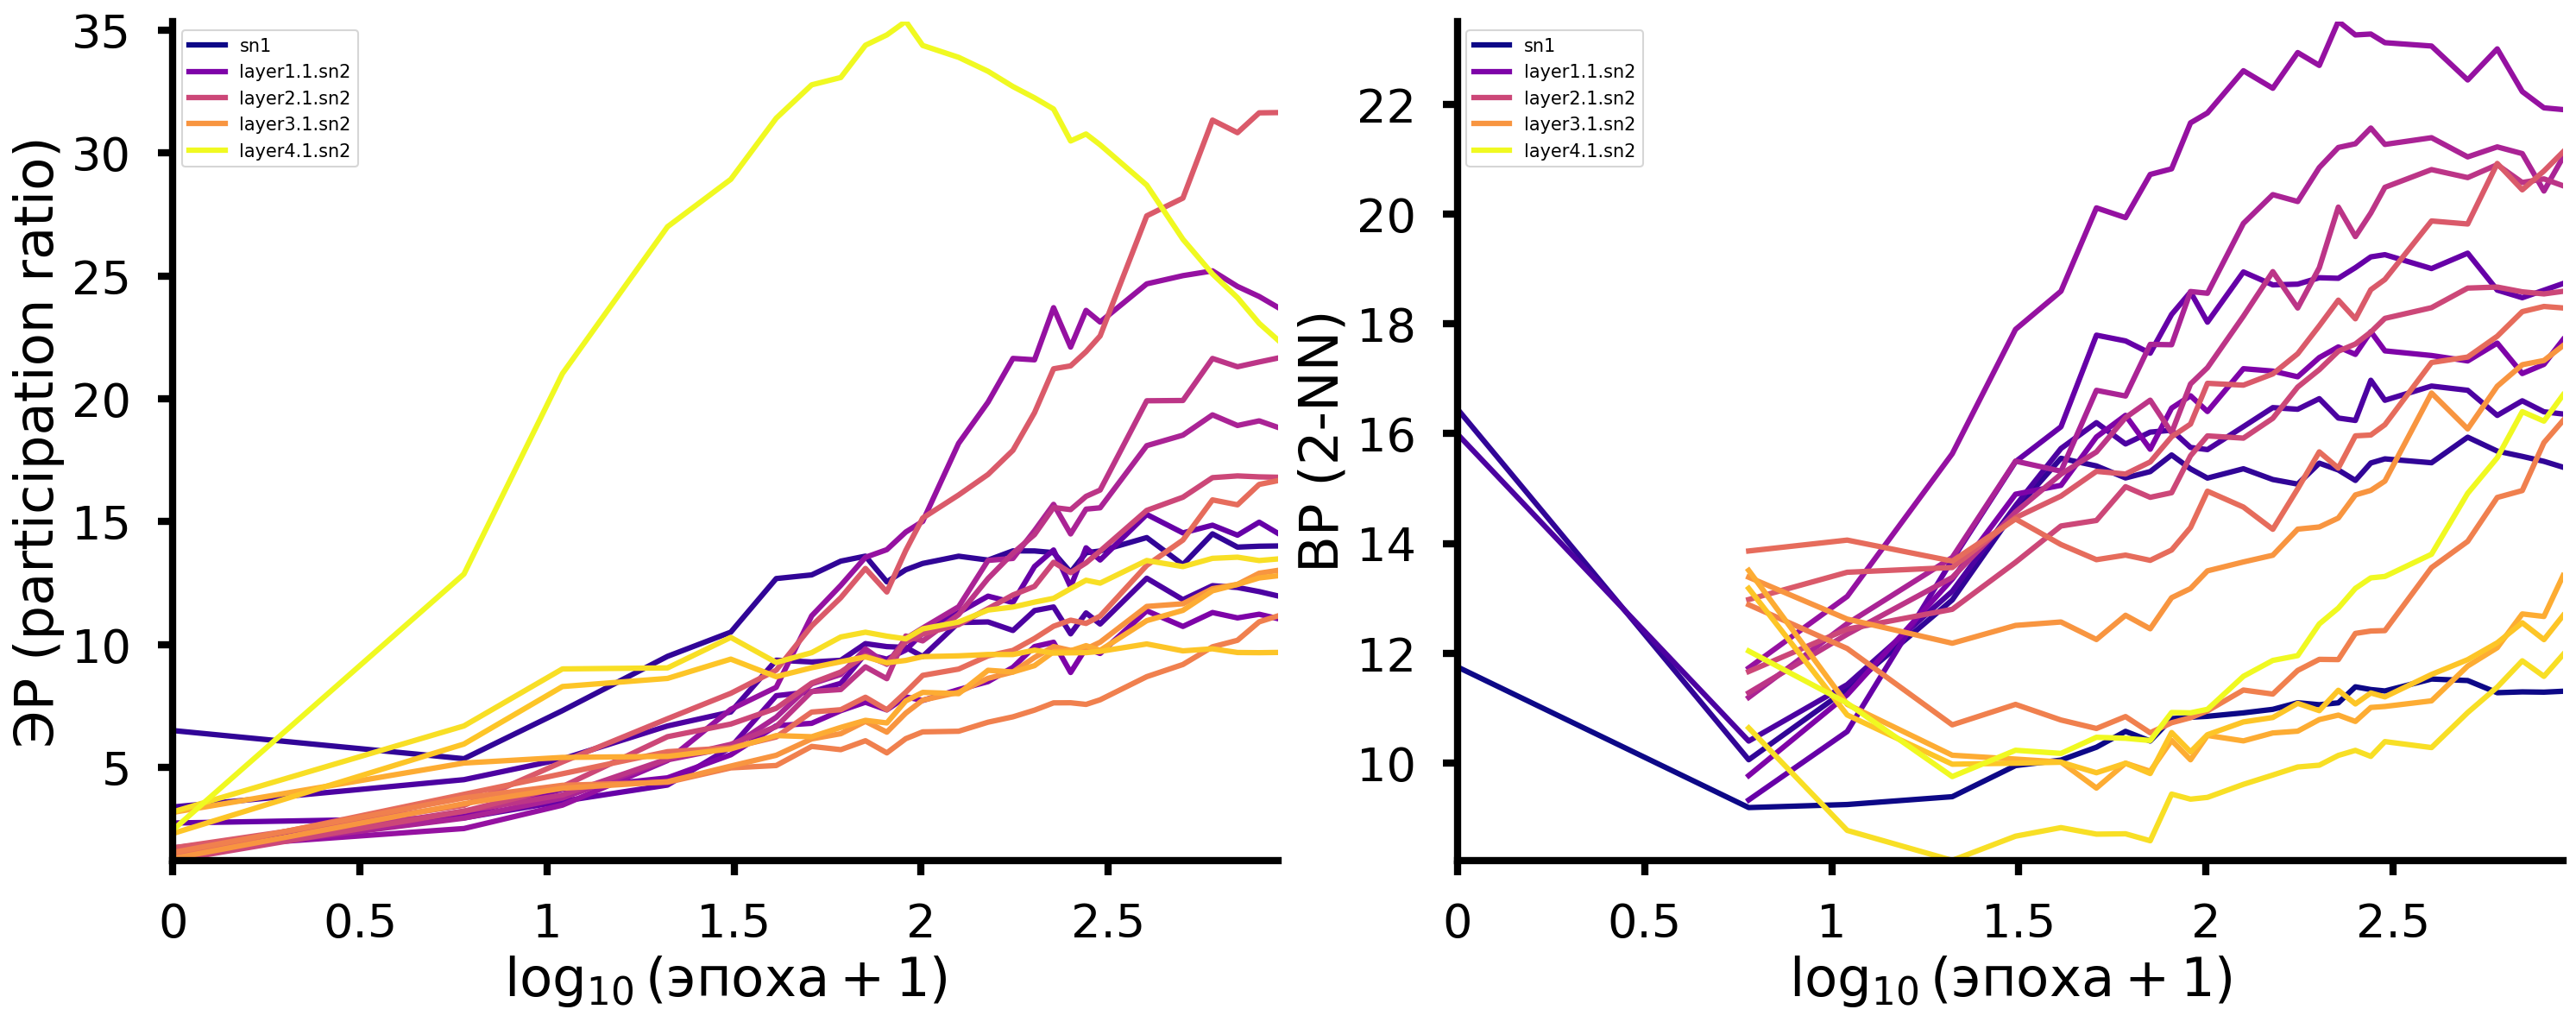
\includegraphics[width=0.95\textwidth]{images/neurotrain/dimensionality_curves.png}
\caption{Внутренняя размерность (ВР) по эпохам обучения для различных слоёв. В глубоких слоях (layer3--4) наблюдается V-образная динамика: начальное сжатие (минимум на эпохах~20--70) сменяется расширением. В ранних слоях ВР монотонно растёт.}
\label{fig:ib_dim_epochs}
\end{figure}

Двухфазная динамика допускает следующую интерпретацию: на начальном этапе сеть сжимает многообразие активности, отбрасывая нерелевантные вариации; после достижения минимума представление усложняется, формируя тонкую дифференциацию между классами. Это согласуется с теоретической работой Recanatesi et al.~\cite{Recanatesi2019}, описавшей два конкурирующих механизма в глубоких сетях~--- расширение и сжатие. LIF-нейрон реализует жёстко пороговую нелинейность, которая по логике Saxe et al.~\cite{Saxe2018} должна способствовать сжатию~--- что и наблюдается.


%========================================================================
\subsection{Информационный анализ представлений}\label{sec:ib_info}

Взаимная информация $I(Z; Y)$ между латентным представлением слоя и метками классов также показывает по слоям профиль в форме горба: рост от sn1 (${\approx}\,0$ бит) к layer3 (${\approx}\,2{,}3$ бита) и падение к layer4 (${\approx}\,1{,}9$ бита). Горб формируется в процессе обучения: на ранних эпохах профиль практически плоский (рис.~\ref{fig:ib_iplane}, нижний ряд справа).

Профили ВР и $I(Z; Y)$ имеют одинаковую форму, но их пики не совпадают по положению, и сопоставление обнаруживает временну\'ю асимметрию между геометрией и классовой информацией. Пик ВР по глубине стабилизируется рано~--- на слоях L2.0--L2.1 уже к эпохе~30~--- и далее не смещается. Пик $I(Z; Y)$, напротив, формируется позже (различим с эпохи~30) и систематически дрейфует вглубь сети: его положение, отслеживаемое по вершине параболической аппроксимации послойного профиля, смещается от L2.1 при эпохе~30 к L3.1 при эпохах~700--900 (${+}2{,}8$ слоя на декаду эпох обучения, коэффициент корреляции $r = 0{,}98$ между положением вершины и $\log_{10}$ эпохи). Геометрическая сложность представления, таким образом, оформляется в промежуточных слоях раньше, чем туда же смещается максимум классовой информации: глубокие слои уточняют задаче-релевантную информацию поверх уже стабилизировавшейся геометрии. Kamkari et al.~\cite{Kamkari2023} теоретически связали внутреннюю размерность и энтропию представлений; совпадение формы профилей служит эмпирической иллюстрацией этой связи, а рассогласование положения пиков уточняет её, разделяя геометрический и информационный аспекты во времени обучения.

Рост $I(Z; Y)$ с глубиной от sn1 к layer3 может казаться противоречащим неравенству обработки данных (DPI), запрещающему рост MI в марковской цепочке. Однако остаточные связи (skip connections) в ResNet нарушают структуру простой цепочки, а $I(Z; Y)$ является нижней границей, качество которой зависит от сложности данных слоя. Падение $I(Z; Y)$ от layer3 к layer4, напротив, представляет реальную потерю уникальной информации, согласованную с ростом избыточности.

На информационной плоскости (рис.~\ref{fig:ib_iplane}, верхний ряд) слои демонстрируют характерные траектории. Промежуточные слои (layer2--3) движутся вправо-вверх~--- оба показателя растут одновременно (фаза подгонки, fitting, по терминологии Shwartz-Ziv и Tishby~\cite{ShwartzZiv2017}). В глубоких слоях layer4, напротив, $H_{gauss}(T)$ сначала растёт, достигая пика на эпохах~70--125, а затем разворачивается влево~--- фаза сжатия: сеть сжимает общую информацию в выходном слое, удерживая $I(Z; Y)$. Величина сжатия нарастает с глубиной: падение $H_{gauss}$ от пика к эпохе~900 составляет ${\approx}\,140$ бит в layer4.0 и ${\approx}\,320$ бит в layer4.1. Разворот на информационной плоскости согласуется с V-образной динамикой ВР: минимум ВР в глубоких слоях (эпохи~20--70) приходится на фазу разворота. Два независимых метода~--- геометрический (ВР) и информационно-теоретический ($H_{gauss}$)~--- дают одну картину. Shwartz-Ziv и Tishby~\cite{ShwartzZiv2017} показали информационную плоскость для малых tanh-сетей; Saxe et al.~\cite{Saxe2018} установили, что сжатие зависит от типа нелинейности. В импульсной сети LIF-нейроны не имеют гладкого насыщения (как tanh), но число спайков ограничено сверху (${\leq}\, T = 50$), что ограничивает информационную ёмкость слоя аналогичным образом.

\begin{figure}[ht]
\centering
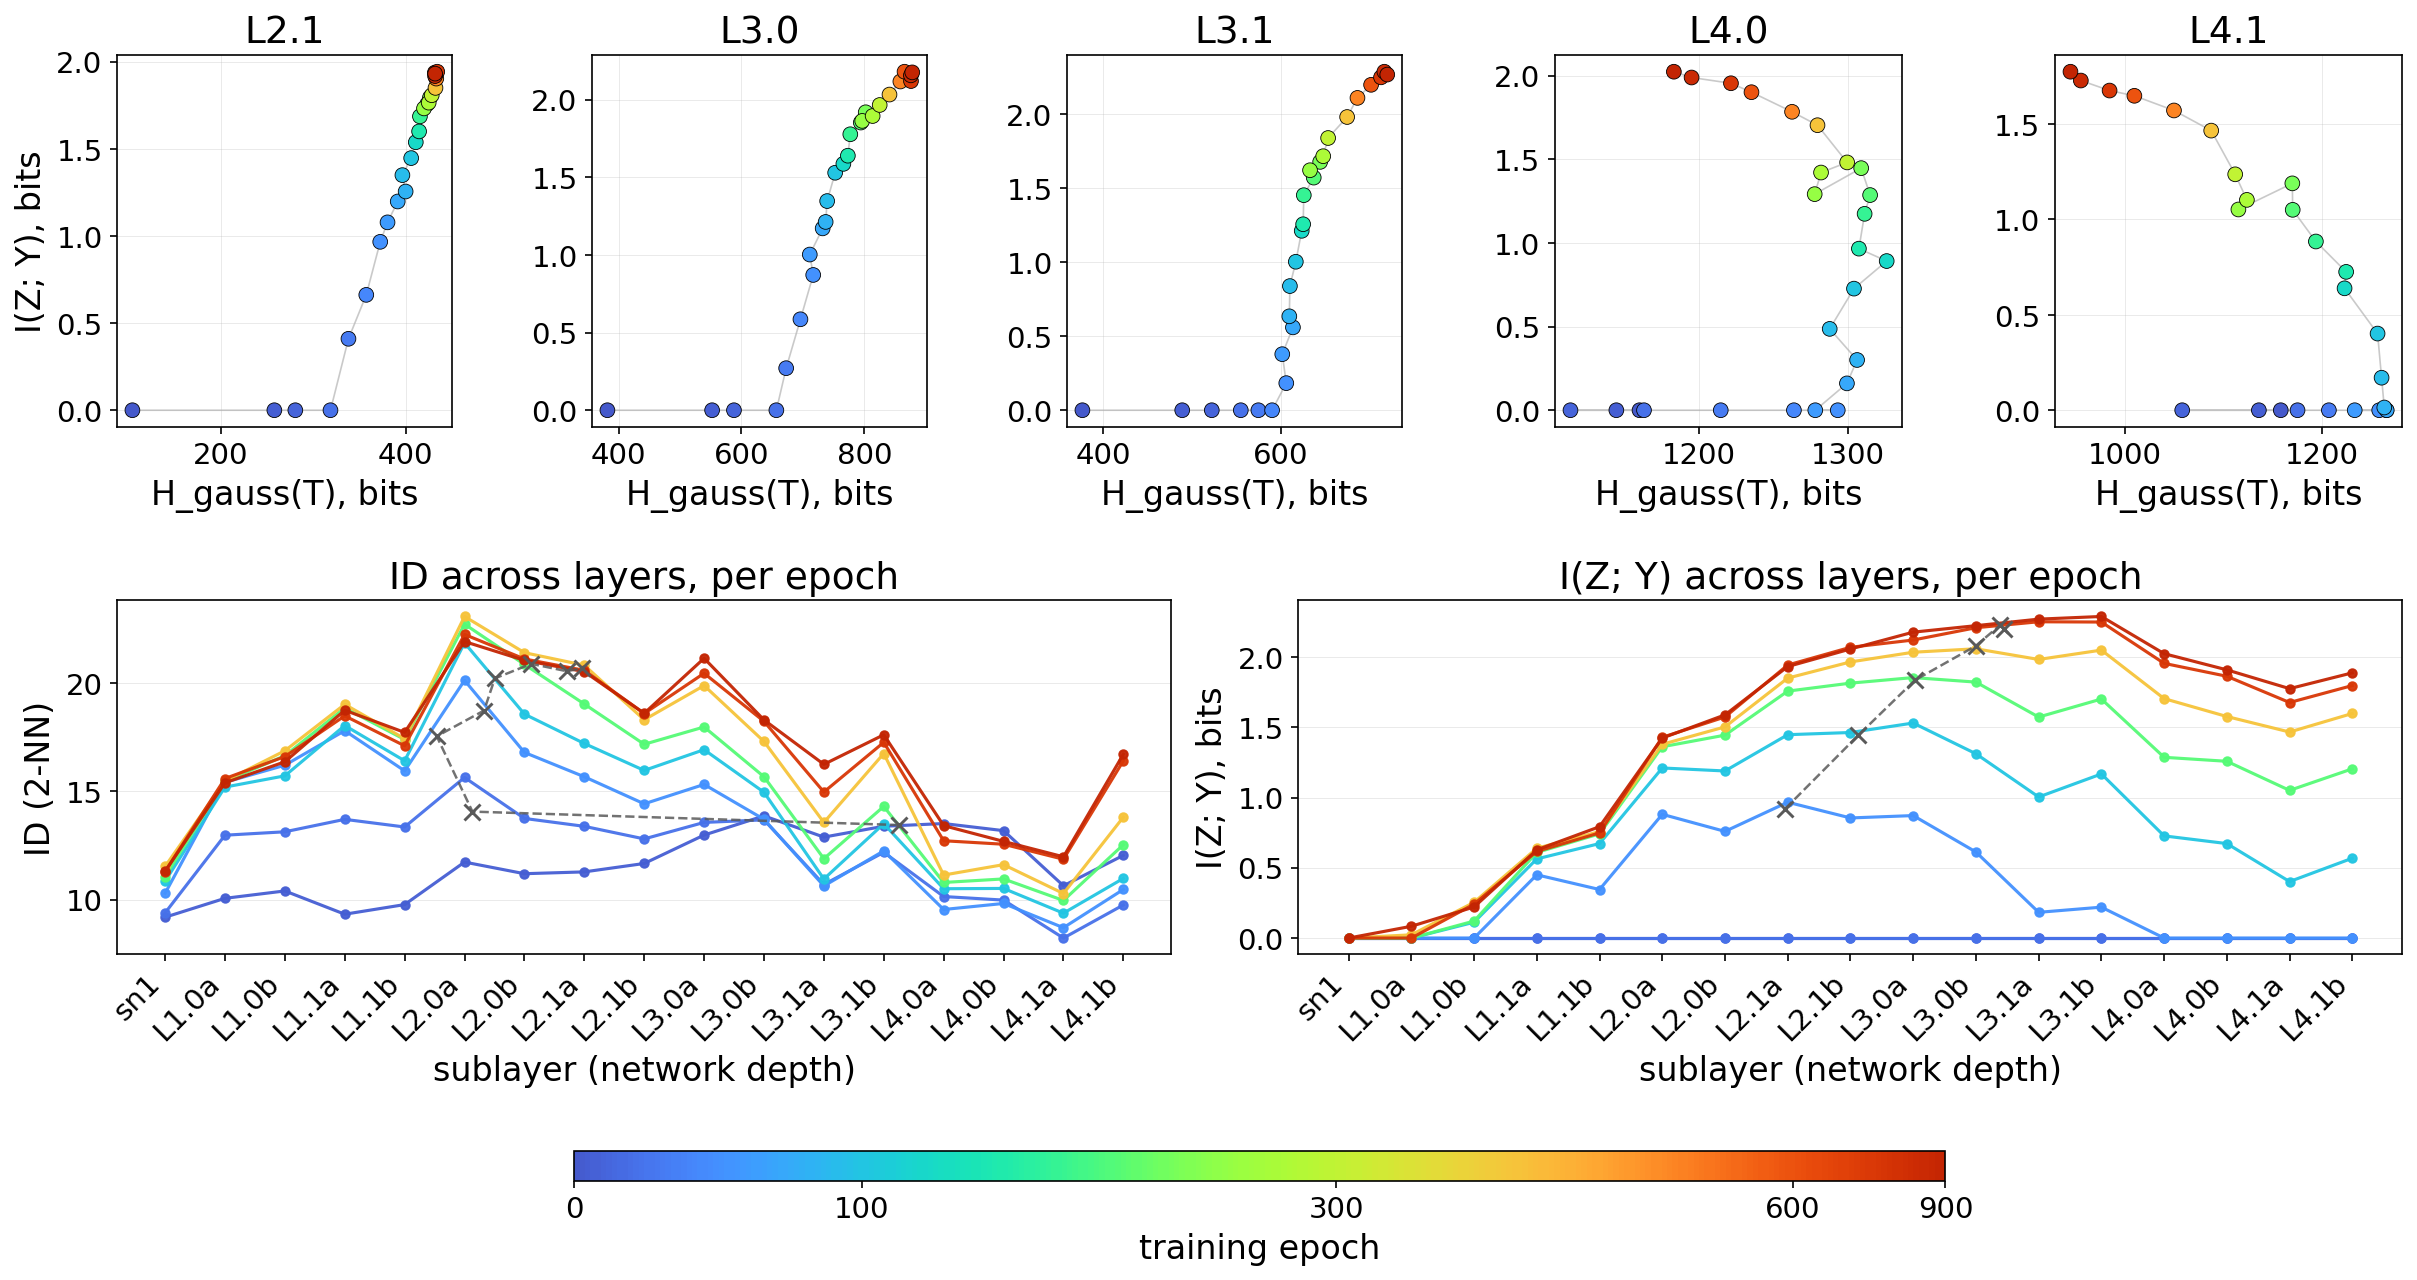
\includegraphics[width=\textwidth]{images/neurotrain/ib_snn_iplane.png}
\caption{Динамика представлений импульсной ResNet-18 в информационной плоскости. \textbf{Верхний ряд:} траектории $I(Z; Y)$ против $H_{gauss}(T)$ для пяти слоёв вдоль глубины сети (L2.1--L4.1); каждая точка~--- одна эпоха обучения, точки соединены хронологически, цвет кодирует эпоху. В промежуточных слоях траектории направлены вправо-вверх (подгонка), в глубоких слоях layer4~--- разворот влево (сжатие). \textbf{Нижний ряд:} послойные профили внутренней размерности (ВР, слева) и $I(Z; Y)$ (справа) для восьми эпох обучения ($e = 5\ldots900$). Серые крестики и пунктир~--- положение вершины параболической аппроксимации профиля: пик ВР стабилизируется рано на L2.0--L2.1, тогда как пик $I(Z; Y)$ дрейфует вглубь сети, к L3.1.}
\label{fig:ib_iplane}
\end{figure}

Для полноты картины в таблице~\ref{tab:ib_summary} сведены три меры для обученной сети.

\begin{table}[ht]
\centering
\caption{Согласованность геометрических и информационных мер представлений импульсной сети}
\label{tab:ib_summary}
\begin{tabular}{lll}
\toprule
\textbf{Мера} & \textbf{По слоям (эп.~900)} & \textbf{По эпохам (layer4)} \\
\midrule
ВР (2-NN) & горб: пик L2, спад L4 & V-образная: мин.~эп.~20--70 \\
$I(Z;Y)$ (KSG) & горб: пик L3, спад L4 & рост $\to$ плато \\
$H_{gauss}$ & рост с глубиной & рост $\to$ спад (сжатие) \\
\bottomrule
\end{tabular}
\end{table}

Сумма попарных MI отдельных нейронов $I_{ind} = \sum_i I(t_i; Y)$ многократно превышает $I(Z; Y)$ во всех слоях и на всех эпохах. В layer4 при эпохе~900 $I_{ind}$ достигает $300{+}$ бит, тогда как $I(Z; Y) \approx 1{,}9$ бита при $H(Y) = \log_2 10 \approx 3{,}32$ бита~--- нейроны выходного слоя массово дублируют классовую информацию. Отношение $I_{gauss}/I_{ind} < 1$ повсюду, что указывает на преобладание избыточного кодирования. Следует отметить, что гауссово приближение $I_{gauss}$ тем грубее, чем сильнее распределение числа спайков отклоняется от нормального; в глубоких слоях с большим числом нейронов ($N = 512$, layer4) количественные значения отношения следует интерпретировать с осторожностью.

Устойчивость результатов проверена тремя контролями. Во-первых, анализ $I(Z; Y)$ повторён с размерностью латентного пространства $d = 8$ (вместо $d = 16$): горб $I(Z; Y)$ по слоям сохраняется (пик в layer3~--- $2{,}57$ бит при $d{=}8$ против $2{,}29$ при $d{=}16$; падение к layer4~--- $2{,}42$ против $1{,}89$), как и разворот на информационной плоскости. Во-вторых, автоэнкодер переобучен в неконтролируемом режиме ($\lambda = 0$, без классификационного лосса): оценки $I(Z; Y)$ при $\lambda = 0$ и $\lambda = 1$ коррелируют с $r \geq 0{,}998$ во всех слоях, а слой-горлышко layer3.1 остаётся пиком в обоих режимах~--- наблюдаемая динамика не является артефактом классификационной задачи автоэнкодера. В-третьих, гауссова оценка $H_{gauss}(T)$ для дискретного числа спайков проверена дитизацией (добавлением равномерного шума): поправка сдвигает значения менее чем на $7\%$ и не меняет ни направления, ни эпохи разворота в layer4.

Методы оценки размерности (ЭР, ВР), применённые здесь к активности импульсной сети,~--- те же, что использовались при анализе кальциевой активности нейронов гиппокампа (секция~\ref{sec:dim}). В обоих случаях внутренняя размерность существенно ниже эффективной, указывая на нелинейную структуру многообразия, и линейные меры не улавливают эффекты, видимые через ВР. Это свидетельствует о субстрат-независимости разработанного инструментария: методы, созданные для анализа биологических нейронных данных, содержательно применимы к искусственным нейронным сетям. Как описанная коллективная динамика представлений связана с формированием индивидуальных специализаций отдельных нейронов, рассматривается далее~--- при анализе синтеза оптимальных стимулов (секция~\ref{sec:ib_mei}).
